\section{Windowless Gaseous Tritium Source}
\label{sec:katrinExpSetupWGTS}
\begin{figure}
    \centering    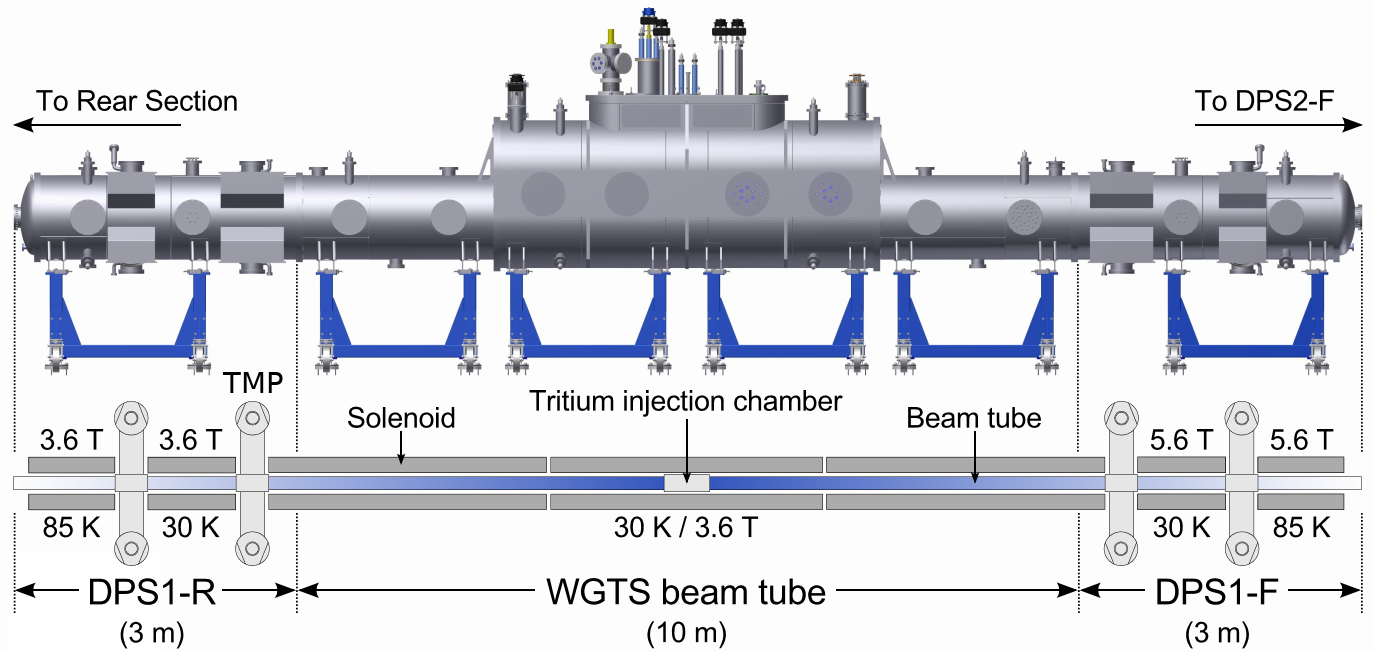
\includegraphics[width=\textwidth]{\currentFigureFolder/wgtsWithTMPLabel.png}
    \xcaption{KATRIN \glsentryfull{wgts}}{The \glsentryfull{wgts}.}{The hull and a sketch of the beam tube are shown. Indicated are the 8 turbo molecular pumps (TMP), the 7 magnets, the design temperatures for tritium operation, the maximum magnetic field strengths and a gradient within the beam tube depicting the decreasing gas density from the center to the sides. (Adapted from \cite{Harms2015}.)}
    \label{fig:katrinExpSetupWGTS}
\end{figure}%
The \gls{wgts} is a 16-m-long, 1.5-m-wide and 4-m-high cryostat. It is depicted in figure \ref{fig:katrinExpSetupWGTS} and a detailed description can e.\,g.~be found in \cite{Grohman2008}. In the following the major features of the \gls{wgts} are reviewed:

{\par\textbf{Tritium purity:} 
The molecular tritium (\ce{T2}) is injected in the middle of the 10-m beam tube of \SI{90}{mm} diameter, where it decays. The design gas column density is $\rho d = \SI{5e17}{molecules/{cm}^2}$ with an isotropic tritium purity of $\epsilon_\text{T} = \SI{95}{\percent}$~\cite{Angrik:2005ep}. At the front and rear of the \gls{wgts}, the gas is extracted from the beam tube by turbo molecular pumps in designated differential pumping sections called DPS-1-R (rear) and DPS-1-F (front). The extracted gas is re-injected in the center of the beam tube. The respective pipe system is called the inner loop~\cite{PRIESTER201542}. The tritium purity $\epsilon_\text{T}$ must be kept stable on a \SI{0.1}{\percent} level~\cite{Angrik:2005ep}. Therefore, a permeator is installed that separates impurities (like e.\,g.~helium) and ejects them into the exhaust loop of the \gls{tlk}. Furthermore, the isotopic composition of the gas
is monitored by a designated \gls{lara}~\cite{Schloesser2013}.}

{\par\textbf{Injection pressure:}
The design injection pressure of the tritium gas is $1.8\text{\,mbar}\mathcal{l}/\text{s}$. It must be kept stable at the $\SI{0.1}{\percent}$ level. This is achieved via a pressure- and temperature-controlled buffer vessel within the inner loop~\cite{PRIESTER201542}.}

{\par\textbf{Magnetic field:}
In order to adiabatically guide the $\upbeta$ electrons to the spectrometer section the \gls{wgts} is submerged in a magnetic field parallel to its beam tube of up to \SI{5.6}{T}. It is created by 7 superconducting coils, that surround the beam tube. These magnets are kept at a temperature of \SI{4.2}{K} by liquid helium~\cite{Arenz2018}.}

{\par\textbf{Temperature:}
On the one hand, thermal motion smears the energy spectrum of the $\upbeta$ electrons (Doppler effect). On the other hand, at low temperatures the gas molecules cluster. $T=\SI{30}{K}$ is chosen as a compromise and established by a two-phase neon cooling system. For calibration purposes, it is also possible to operate the \gls{wgts} with krypton-83m instead of tritium. This requires a beam tube temperature of $T=100K$ in order for the krypton not to freeze. In this operational mode the neon has to be exchanged for argon~\cite{Angrik:2005ep}.}
